\documentclass[a4paper]{scrartcl}

\usepackage[english]{babel}
\usepackage[utf8]{inputenc}
\usepackage{times}
\usepackage{graphicx}
\usepackage{url}
\usepackage[colorinlistoftodos]{todonotes}
\usepackage{multicol}
\usepackage{wrapfig}

% Look for images in ./images folder.
\graphicspath{{./images/}}

% Front page main information.
\title{\gamename}
\subtitle{Game Design Document}
\author{}
\date{\today}

\begin{document}

% Define the name of the game.
\newcommand{\gamename}{\emph{Ice Cream Factory}}

\maketitle

\section{About the game}
    In \gamename, you are responsible for assembling an ice cream production
    line. You must place the right machines along the conveyor belt and fill the
    orders correctly. But don't think this is going to be an easy task. You must
    find out clever solutions in order to produce the right types of ice cream
    with only a few devices path changers. Prepare yourself to face a delicious
    series of mind blowing puzzles.

\section{Description}
    Produce ice cream is a sweet business. So many flavors, so many toppings, so
    many combinations! Your job in \gamename is to plan the factory production
    line in such a way that only the right combinations are made.

    In each stage you will have a limited number of devices and a list ice cream
    types that your factory needs to produce. You must find a way of fulfill the
    stage requirements by placing path-changing devices, ice cream dosers and
    other machines along the conveyor belt.

    The belt fed with vessels which will travel all the way to the freezer. When
    a vessel reach a device, the machine will perform an action according to its
    type.

    \subsection{Input machines}
        The production line needs to be fed with items which will hold the ice
        cream. Without them our precious product would be spilled all over the
        place. To avoid that, usually the start point of the conveyor belt will
        have at least one device able to put on the line one of the following
        containers:

        \subsubsection{Ice cream pint}
            \begin{minipage}[t][2em][t]{\textwidth}
                \begin{wrapfigure}{l}{0.1\textwidth}
                    \vspace{-15pt}
                    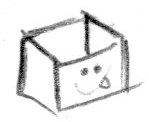
\includegraphics[scale=1]{devices/pint}
                    \vspace{-20pt}
                \end{wrapfigure}

                Vessel for the regular ice cream. In some stages, the pint may have
                a bigger volume in order to be compatible with multiple runs through
                dosers.
            \end{minipage}

        \subsubsection{Popsicle molds}
            \begin{minipage}[t][3em][t]{\textwidth}
                \begin{wrapfigure}{l}{0.1\textwidth}
                    \vspace{-15pt}
                    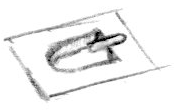
\includegraphics[scale=1]{devices/popsicle_molds}
                    \vspace{-25pt}
                \end{wrapfigure}

                Mold and stick for popsicle. There is no need to use special
                different dosers to make popsicle. Don't worry.
            \end{minipage}

        \subsubsection{Banana plate}
            \begin{minipage}[t][2em][t]{\textwidth}
                \begin{wrapfigure}{l}{0.1\textwidth}
                    \vspace{-20pt}
                    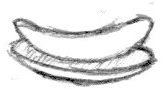
\includegraphics[scale=1]{devices/banana_plate}
                    \vspace{-25pt}
                \end{wrapfigure}

                Special container to make bana-split.
            \end{minipage}

    \subsubsection{Action machines}
        The action machines are responsable to bring joy to the production line.
        In other words, these are the devices that fill the containers with
        icecream and cover them with toppings.

        \subsubsection{Ice cream doser}
            \begin{minipage}[t][6em][t]{\textwidth}
                \begin{wrapfigure}[5]{l}{0.16\textwidth}
                    \vspace{-20pt}
                    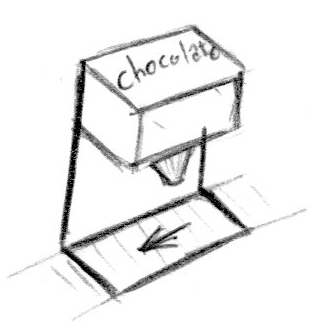
\includegraphics[scale=1]{devices/ice_cream_doser}
                    \vspace{-20pt}
                \end{wrapfigure}

                Pours ice cream into vessels under this device;\\
                Works for pints, popsicle molds and banana plates the same way;\\
                Each doser can use any flavor, but it is only possible to change
                flavors when the production line is not running.
            \end{minipage}

        \subsubsection{Topping doser}
            \begin{minipage}[t][6em][t]{\textwidth}
                \begin{wrapfigure}[5]{l}{0.16\textwidth}
                    \vspace{-20pt}
                    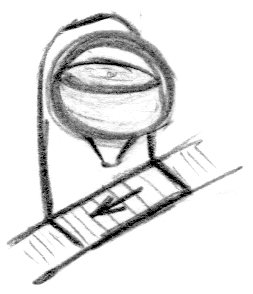
\includegraphics[scale=1]{devices/topping_doser}
                    \vspace{-10pt}
                \end{wrapfigure}

                Works the same way ice cream doser does, but topping flavors are
                note the same.
            \end{minipage}

        \subsubsection{Special topping doser}
            \begin{minipage}[t][6em][t]{\textwidth}
                \begin{wrapfigure}{l}{0.2\textwidth}
                    \vspace{-20pt}
                    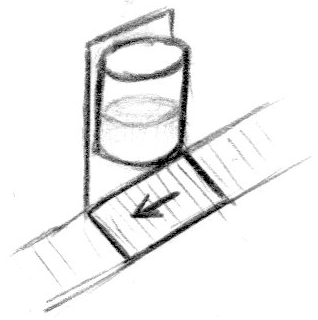
\includegraphics[scale=1]{devices/special_topping_doser}
                    \vspace{-20pt}
                \end{wrapfigure}

                Also work the same way the other dosers, but pour candies and
                other special candies.
            \end{minipage}

    \subsection{Control machines}
        $[$JUST RANDOM WORDS - TO BE IMPROVED$]$

        Besides stacking ice cream pieces, it is important to manage the path
        each item will follow inside your factory.
        Big part of puzzle solving.
        Can be a great challenge because most of the time you will have a
        limited number of devices to achieve a goal.

        \subsubsection{Switcher}
            \begin{minipage}[t][4em][t]{\textwidth}
                \begin{wrapfigure}{l}{0.2\textwidth}
                    \vspace{-20pt}
                    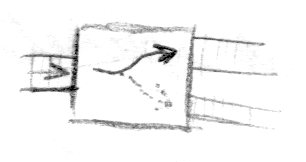
\includegraphics[scale=1]{devices/switcher}
                    \vspace{-15pt}
                \end{wrapfigure}

                The switcher is the simplest path control machine. One conveyor
                track comes in but two goes out. The first item that gets into
                this is driven to a track, the second item is driven to the
                other track, and the third item is driven again to the first
                track.
            \end{minipage}

        \subsubsection{Joint}
            \begin{minipage}[t][3em][t]{\textwidth}
                \begin{wrapfigure}{l}{0.2\textwidth}
                    \vspace{-20pt}
                    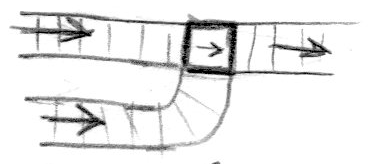
\includegraphics[scale=1]{devices/joint}
                    \vspace{-20pt}
                \end{wrapfigure}

                Using the Switcher will create a branch in your production line.
                If you want to reconnect two tracks back into one, just put a
                joint.
            \end{minipage}

        \subsubsection{Weighing Scale}
            \begin{minipage}[t][8em][t]{\textwidth}
                \begin{wrapfigure}{l}{0.2\textwidth}
                    \vspace{-20pt}
                    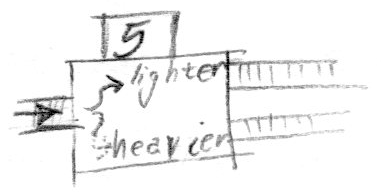
\includegraphics[scale=1]{devices/scale}
                    \vspace{-20pt}
                \end{wrapfigure}

                The scale is very similar to the switcher, with one track going
                in and two going out. But instead of leading items to alternated
                paths, this machine chooses the output track according to the
                weight of the item. If the measured weight is greater than a
                defined value, the item goes to the ``heavier'' track. Otherwise
                the item is driven to the ``lighter'' track.

                You can set any comparison value you wish. It worth noticing
                that ice cream is heavier than regular topping, which is heavier
                than special topping, which is heavier than special topping.
            \end{minipage}

        \subsubsection{Taster}
            \begin{minipage}[t][3em][t]{\textwidth}
                \begin{wrapfigure}{l}{0.24\textwidth}
                    \vspace{-20pt}
                    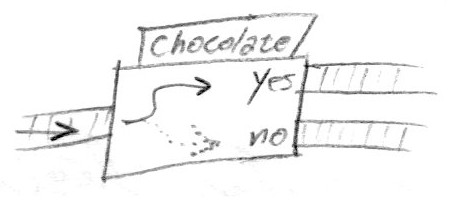
\includegraphics[scale=1]{devices/taster}
                    \vspace{-20pt}
                \end{wrapfigure}

                This device checks whether the ice cream flavor is the same of a
                specified one. If it is, the item goes to ``yes'' track. If it
                is not or if the vessel is empty, the item goes to ``no'' track.
                You can set the verification flavor the same way done with the
                weighing scale.
            \end{minipage}

        \subsubsection{Multi-Taster}
            The Multi-Taster is an advanced version of Taster. Instead of two
            output tracks, this machine can handle as many output tracks as the
            number of available flavors. Each output track corresponds to a
            flavor.

            You can set the machine so that it has fewer output tracks than
            available flavors. But if you use this configuration, you must have
            a ``none of the others'' track.

        \subsubsection{Generic Tester}
            \begin{minipage}[t][6.1em][t]{\textwidth}
                \begin{wrapfigure}{l}{0.45\textwidth}
                    \vspace{-20pt}
                    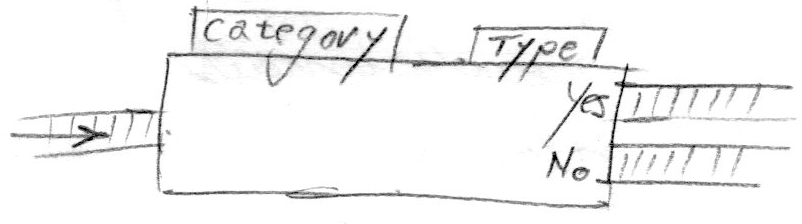
\includegraphics[scale=1]{devices/generic_conditional}
                    \vspace{-20pt}
                \end{wrapfigure}

            The generic tester is the ultimate control machine. With this device
            you can check pretty much any characteristic an item my have.

            This machine requires you to set three parameters: (1) the
            characteristic to be test; (2) the comparison method; (3) the value
            to be compared with.
            \end{minipage}

            For example, you set ``flavor'' in (1) then you can select ``is'' or
            ``is not'' in (2) and all available flavors in (3). You can do the
            same for ``topping'' and ``vessel'' too. If you select ``weigh'' in
            (1), the options in (2) are ``is lower than'', ''is equal to'', or
            ``is greater than''.

    \subsection{Other}
        \subsubsection{Freezer}
            This is the end of line. All tracks must lead to the freezer so the
            ice cream can get ready to the costumers.

        \subsubsection{Synchronizer}
            Every time an item reaches the Synchronizer, this machine stops the
            track (only the current branch) for a while. The number of time
            steps in pause is set by you.

        \subsubsection{Logic Gates}
            In order to use the full potential of control machines you can
            connect them using Logic Gates. The gates are ``AND'' and ``OR''.
            This complex device is intended only for very advanced uses.

\section{Features}
    \begin{itemize}
        \item Over XXX levels;
        \item 3 base ice creams, 4 flavors, 5 toppings, 4 special toppings;
        \item 13 different factory machines;
        \item Mind blowing puzzles;
    \end{itemize}

\section{Target platforms}
    \gamename is a simple and casual game, making it ideal for browser, tablets
    and PC. Player will perform actions through mouse clicking or by touch.

\section{Concept art}
    Here there are a few images to show the visual identity of \gamename.

    \centering
    $[$ TO BE FILLED $]$

\section{Similar games}
    In this section we can see some factory games which have the same conveyor
    concept present in \gamename.

    \begin{multicols}{2}
        \subsection{Cake Factory - Barbie Games}
            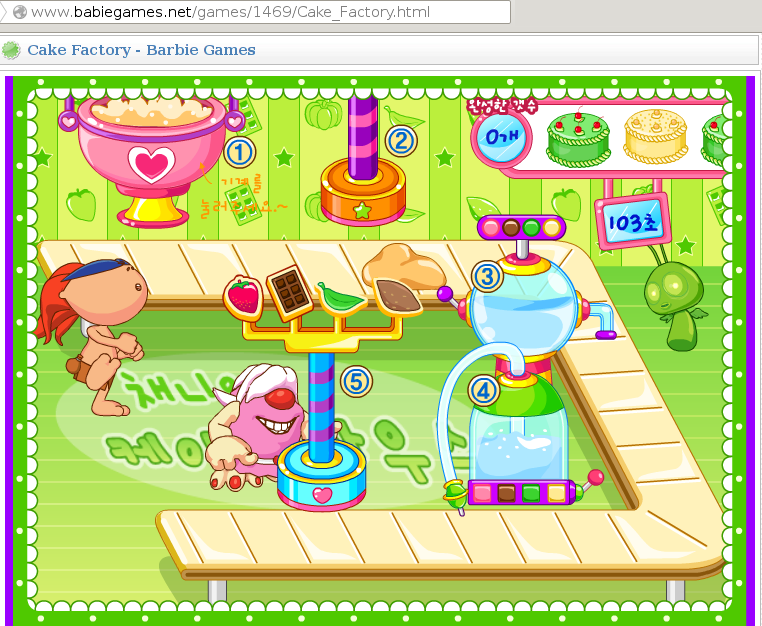
\includegraphics[width=0.49\textwidth]{similar_games/CakeFactory}

        \subsection{Toy Factory Fun}
            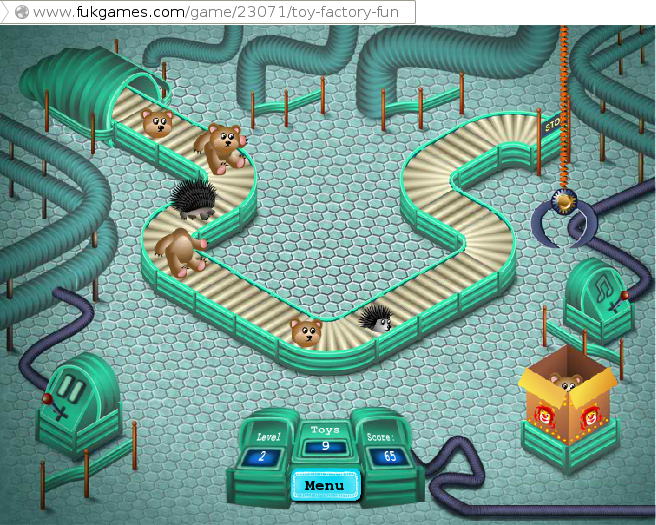
\includegraphics[width=0.49\textwidth]{similar_games/ToyFactoryFun}
    \end{multicols}

    \begin{multicols}{2}
        \subsection{Jewel Factory}
            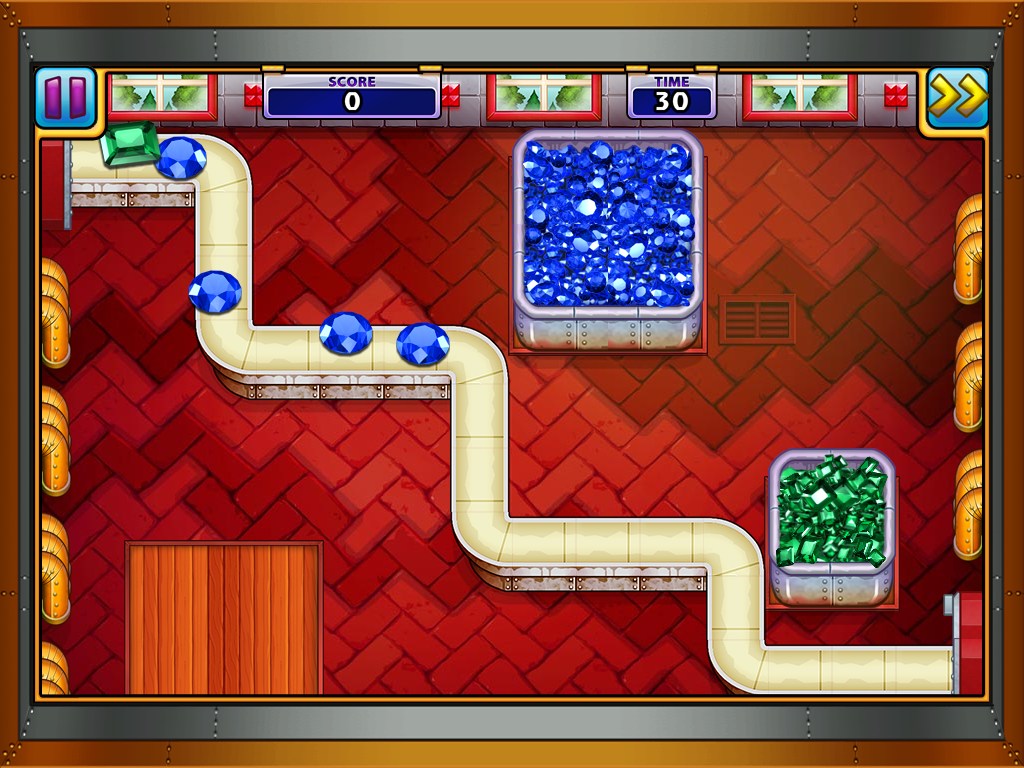
\includegraphics[width=0.49\textwidth]{similar_games/JewelFactory}

        \subsection{Production Panic}
            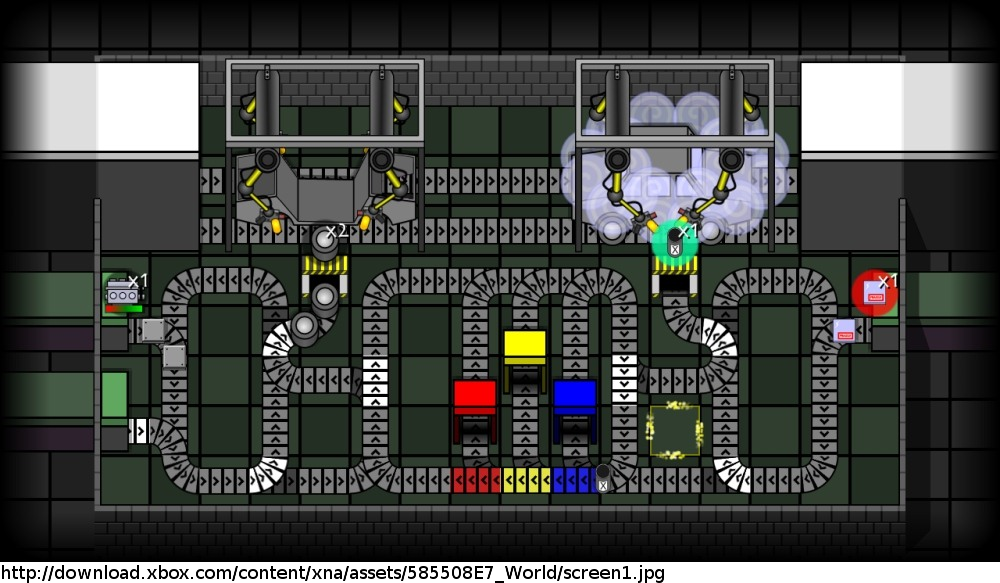
\includegraphics[width=0.49\textwidth]{similar_games/ProductionPanic}
    \end{multicols}

    \begin{multicols}{2}
        \subsection{Candy Factory - LeeGT}
            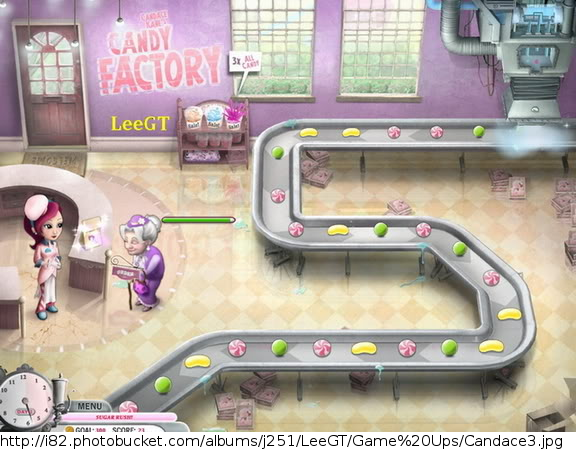
\includegraphics[width=0.49\textwidth]{similar_games/CandyFactoryLeeGT}

        \subsection{Teddy Factory}
            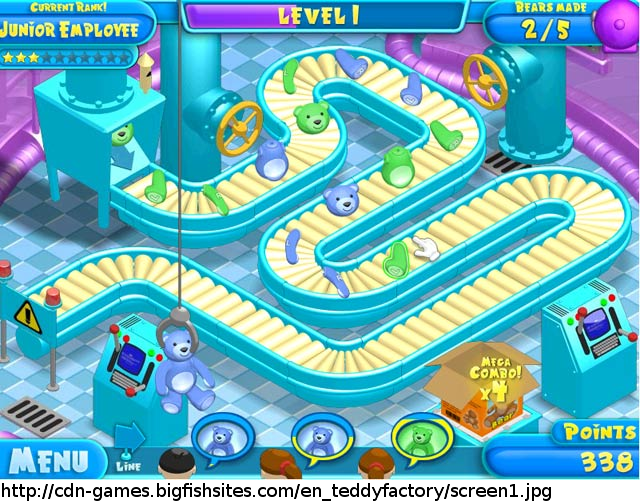
\includegraphics[width=0.49\textwidth]{similar_games/TeddyFactory}
    \end{multicols}

    \begin{multicols}{2}
        \subsection{Robot Factory}
            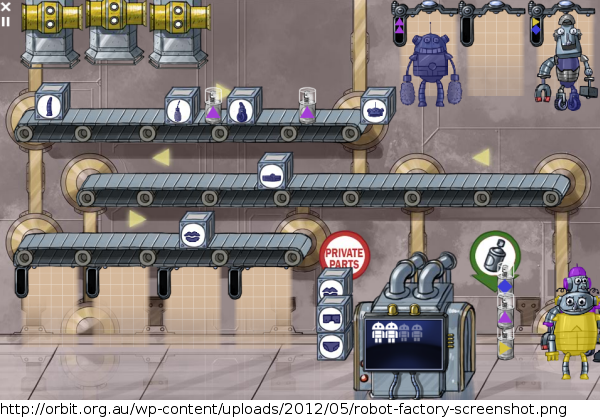
\includegraphics[width=0.49\textwidth]{similar_games/RobotFactory}

        \subsection{Space Chem}
            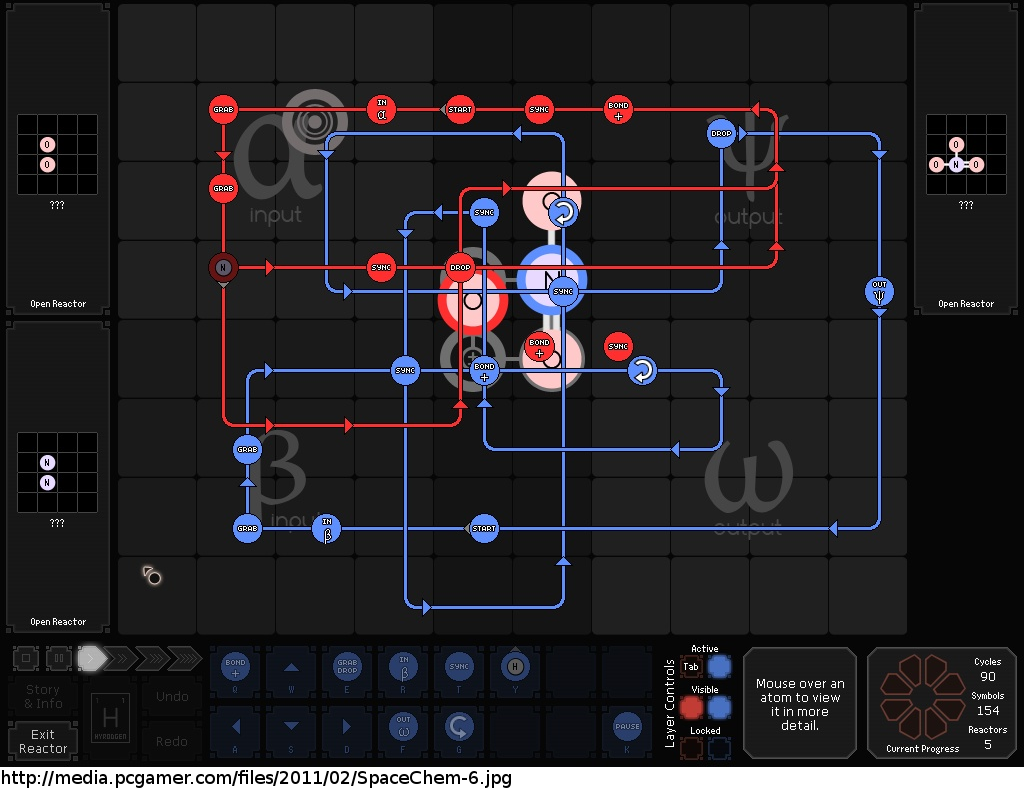
\includegraphics[width=0.49\textwidth]{similar_games/SpaceChem}
    \end{multicols}

\section{Game name alternatives}
    \begin{itemize}
        \item Smart Factory
        \item Smart Cream
        \item Smart Ice Cream Factory
        \item Smart Split
        \item Ice Cream Factory
    \end{itemize}

\end{document}
